\section{Theoretische Grundlagen}
\subsection {Einordnung VR, AR und MR}
%Was ist AR
Bei Augmented Reality (\acrshort{ar}) Anwendungen werden dreidimensionale virtuelle Objekte in eine echte dreidimensionale Umgebung in Echtzeit integriert. Es handelt sich um eine Variation der Virtual Environments (\acrshort{ve}), der Virtuellen Realität (\acrshort{vr}) \cite{Azuma1997}. Gerne wird zwischen \acrshort{ar}, \acrshort{vr} und Mixed Reality (\acrshort{mr}) unterschieden. Speicher und seine Ko-Autoren \cite*{Speicher2019} haben zur Eingrenzung Charakteristiken definiert, die aus Interviews mit Experten hervorgehen. 

%VR
\acrshort{vr} hat die Eigenschaft eine komplett synthetisch generierte, virtuelle Welt darzustellen. So bietet sich die Möglichkeit für den Nutzer unerreichbare Orte zu erleben. Es werden hierfür VR-Headsets wie die Oculus Rift S\footnote{https://www.oculus.com/rift-s/, zuletzt aufgerufen am 27.07.2022} oder die Playstation VR\footnote{https://www.playstation.com/de-de/ps-vr/, zuletzt aufgerufen am 27.07.2022} benötigt und die Bewegung des Headsets muss getrackt\footnote{siehe Kapitel \ref{tracking} \nameref{tracking}} werden. Der Nutzer ist während der VR-Erfahrung von der echten Umgebung isoliert, wodurch die soziale Interaktion gering ist. 

%AR
Zusätzlich zu der Definition Azumas\cite{Azuma1997} von \acrshort{ar} wird die Eigenschaft genannt, dass der virtuelle Content dazu in der Lage ist mit der echten Welt zu interagieren. Im Gegensatz zu \acrshort{vr} ist der Nutzer im gegenwärtigen physischen Raum gebunden. Die menschliche Wahrnehmung wird durch das augmentieren und der Kreation von Content Erfahrungen verbessert\cite{Speicher2019}.

%MR
Die Eingrenzung von \acrshort{mr} ist nicht eindeutig. So wird \acrshort{mr} als Kombination von AR und VR gesehen. Die Anwendungen bieten die Möglichkeit sowohl AR als auch VR zu nutzen. Auch wird Mixed Reality in Verbindung mit spezifischer Hardware wie die HoloLens\footnote{https://www.microsoft.com/de-de/hololens, zuletzt aufgerufen am 27.07.2022} gebracht. Ein weiteres Beispiel ist Pokemon GO\footnote{https://pokemongolive.com/de/, zuletzt aufgerufen am 27.07.2022}, bei dem zwischen der AR Funktion und einer virtuellen Umgebung umgeschaltet werden kann.

In Abbidldung \ref*{fig: RV_Kontinuum} haben Milgram und seine Ko-Autoren eine Grafik definiert, die das \textit{Reality-Virtuality Continuum} darstellt. Die linke Hälfte des Kontinuums repräsentiert jede Umgebung, die rein aus realen Objekten besteht, persönlich betrachtet wird und durch jegliche Art wie den Blick durch ein Fenster oder eines Displays erweitert wird. Die rechte Hälfte besteht aus rein virtuellen Objekten, die entweder Monitor-basierend oder immersiv sind. Durch diese Darstellung wird \acrshort{mr} zwischen diesen beiden Extremen eingeordnet und als Umgebung definiert, die die reale und die virtuelle Welt zusammen in einem Display darstellt \cite{Milgram1995}.

\begin{figure}[H]
    \centering
    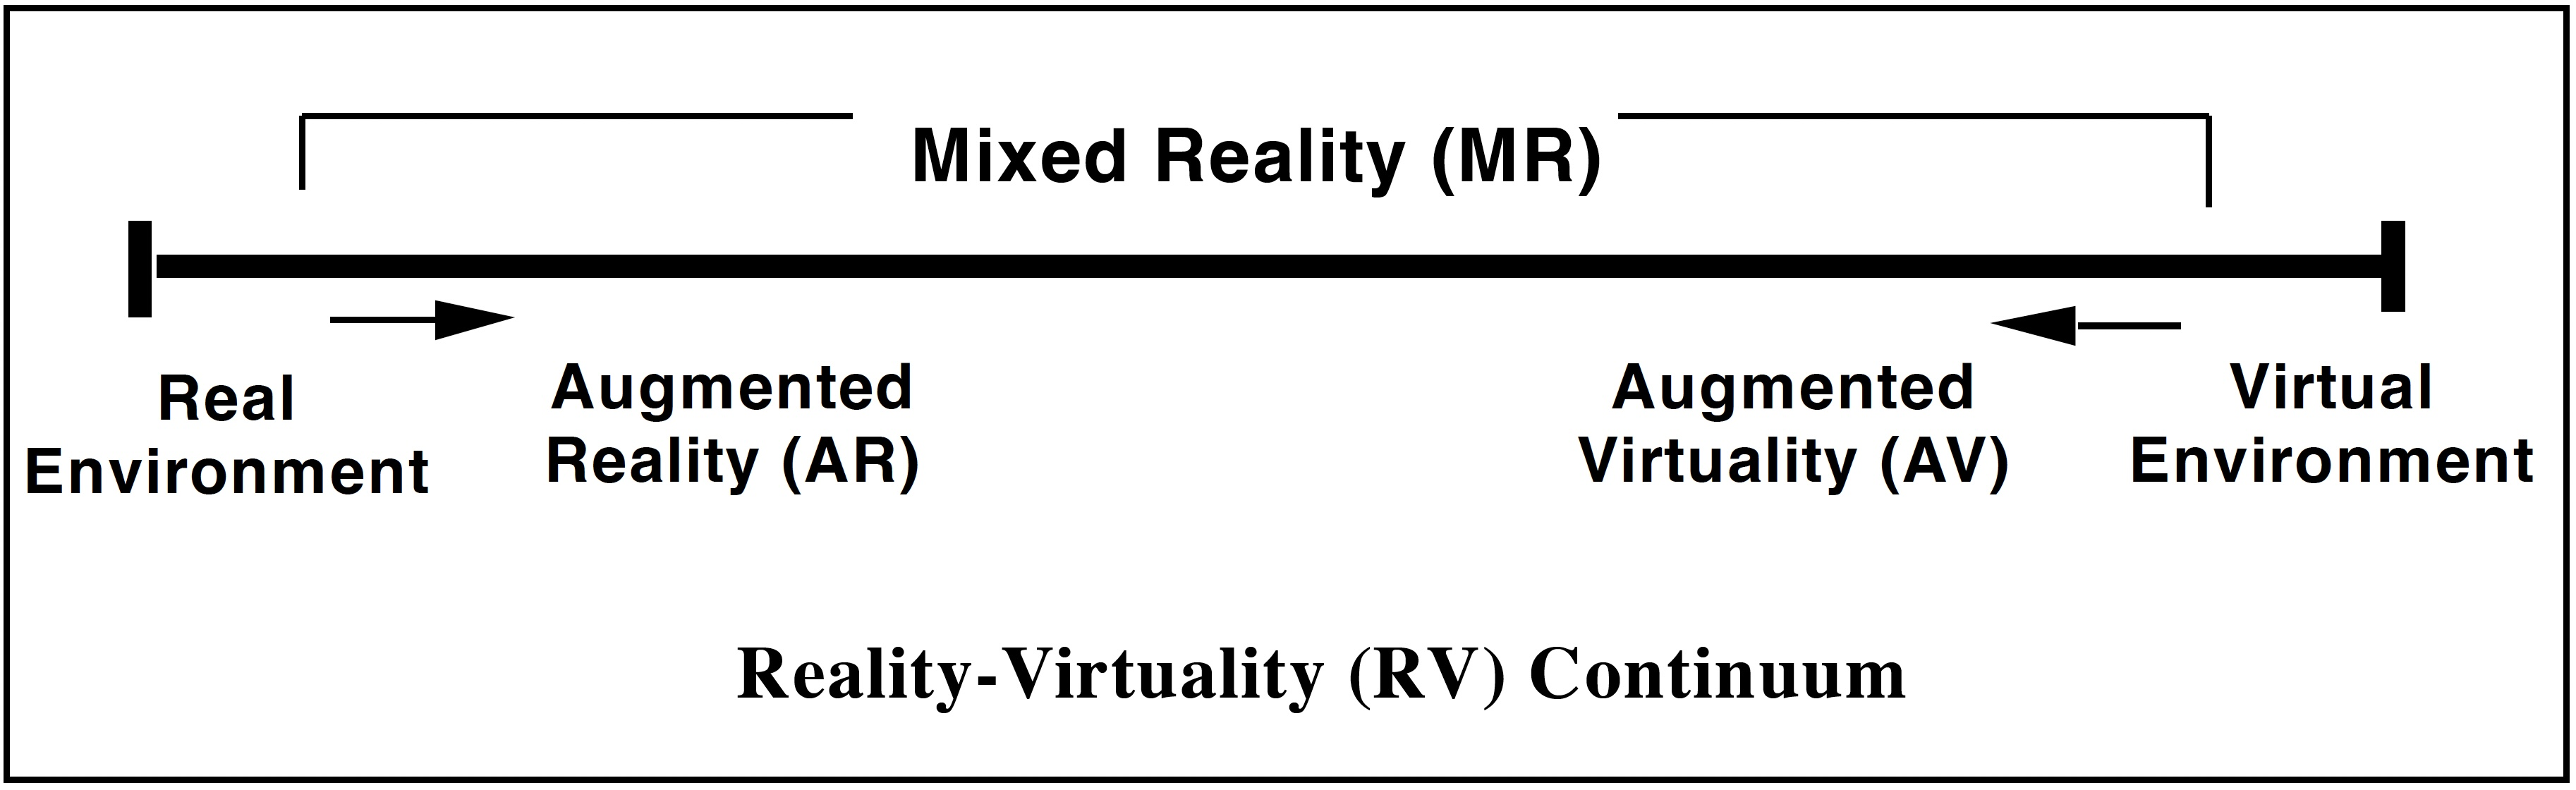
\includegraphics[width=\textwidth]{img/einordnung_vr_ar_mr/vr_ar_mr_kontinuum.jpg}
    \caption{Das Reality-Virtuality Kontinuum nach Milgram\cite{Milgram1995}.}
    \label{fig: RV_Kontinuum}
\end{figure}

Nach diesen Definitionen wird die Anwendung dieser Arbeit in die Augmented Reality eingeordnet. Die virtuellen Objekte in Form der Gebäude werden in die echte dreidimensionale Welt projiziert. Der Nutzer hat die Möglichkeit mit diesen zu interagieren. Jedoch wird es nicht möglich sein den betrachteten Raum zu verlassen und in eine reine virtuelle Welt umzusteigen. 
